\section{LinuX Containers}

\begin{frame}{LinuX Containers Overview}
	\begin{columns}[T]
		\begin{column}{.5\textwidth}
			\begin{itemize}
			\item Features:
				\begin{itemize}
				\item mainline kernel support
				\item application vs. system containers
				\item active development
				\end{itemize}
			\item Components:
				\begin{itemize}
				\item \textit{kernel features}
				\item \textit{userspace tools}
					\begin{itemize} \item binaries, scripts \end{itemize}
				\item \textit{configuration files}
					\begin{itemize} \item container-host interface \end{itemize}
				\item \textit{template files}
					\begin{itemize} \item container applications \end{itemize}
				\end{itemize}
			\end{itemize}
		\end{column}
		\begin{column}{.5\textwidth}
			\begin{figure}[ht]
				\centering
				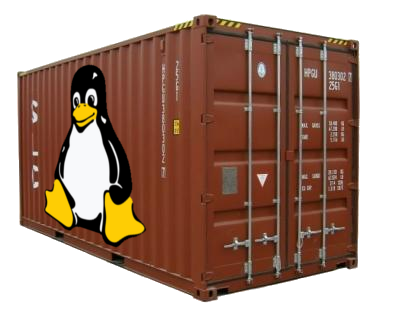
\includegraphics[width=\textwidth]{img/containers.png}
			\end{figure}
		\end{column}
	\end{columns}
\end{frame}

\begin{frame}{Kernel Support}
	\begin{columns}[T]
		\begin{column}{.5\textwidth}
			\begin{itemize}
			\item Namespaces:
				\begin{itemize}
				\item wrap system resources in an abstraction
				\item processes see the resource as their own
				\item isolation between processss in different namespaces
				\end{itemize}
			\item Control Groups
				\begin{itemize}
				\item resource management among processes
				\item hierarchical support
				\item interaction with resource responsible structures:
					\begin{itemize}
					\item the scheduler
					\item the pager
					\end{itemize}
				\end{itemize}
			\end{itemize}	
		\end{column}
		\begin{column}{.5\textwidth}
			\begin{figure}[ht]
				\centering
				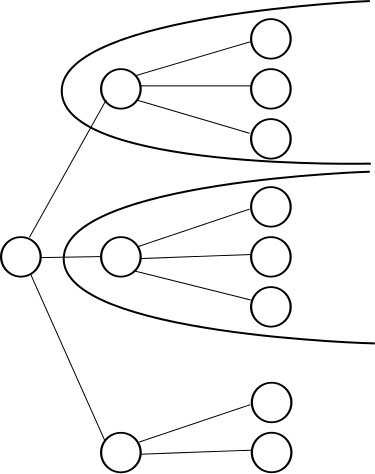
\includegraphics[scale=0.2]{img/namespaces.png}
			\end{figure}
			
			\begin{figure}[hb]
				\centering
				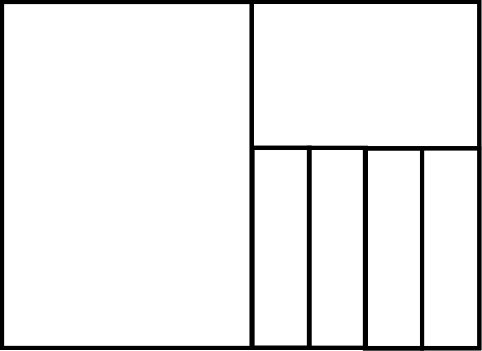
\includegraphics[scale=0.2]{img/cgroups.png}
			\end{figure}
		\end{column}
	\end{columns}
\end{frame}